\chapter{User Study}
\label{ch:Evaluation}

We hypothesized identifying important commits automatically and providing integrated access between commit and issue information could help a developer more effectively access the rationale for code.
To evaluate our hypothesis, we conducted a user study in the form of a semi-structured interview and targeted the following research questions:

\begin{itemize}[leftmargin=*]
    \item[] \RQ{1}{Can we automatically identify the commits that software developers would want to examine?}
    \item[] \RQ{2}{Does highlighting important commits help software developers explore a file’s revision history more efficiently?}
    \item[] \RQ{3}{How useful is direct integration of issue information in the IDE for helping a developer search for code rationale information?}
\end{itemize}

We describe the method we designed to address these research questions in \autoref{sec:Method} 
and present the results of our analysis \autoref{sec:Results}.

%%%%%%%%%%%%%%%%%%%%%%%%%%%%%%%%%%%%%%%%%%%%%%%%%%%%%%%%%%%%%%%%%%%%%%
\section{Method}
\label{sec:Method}

We designed the user study as an explorative, semi-structured interview composed of two parts with an estimated duration of 1 to 1.5 hours.
A semi-structured interview format allows us to maintain a focused discussion while also eliciting interesting responses and reasoning from participants \cite{shull_guide_2007}.
The semi-structured interview format is also appropriate as we seek to understand how participants interact with the commit history for a file and the Intelligent History plugin.
The study involved having participants explore the commit history of two Java classes from the Apache Kafka project to find answers to questions related to motivation and rationale behind changes in the classes.
The briefing for the study and the setup instructions can be found in Appendix \ref{sec:Briefing-and-Setup}.
We expected the participants to interact with commit and issue information found in the commit history in order to be able to answer these questions.

The first part of the user study session consisted of asking questions from two sets of questions about two Java classes from Apache Kafka.
These questions are presented in \autoref{tab:Question-Sets} and require exploring and 
locating particular commits or changes in a given Java class' commit history to try to find code rationale information through inspecting the commits' full commit messages,
diffs, and any relevant Jira issues.
In cases where a Jira issue referenced a Kafka Improvement Proposal (\entity{KIP}), we allowed the participant to visit these \entity{KIP}s in the browser.
Each question set pertains to a different Java class from the Apache Kafka project.
This facilitated an experiment where the participant would complete an initial set of questions without being allowed to use the features of Intelligent History plugin.

After completing the initial provided set of questions, the participant is introduced to the features of the Intelligent History plugin and permitted to use them to help them answer the second set of questions.
The \class{Topology} class for set A contains 22 commits and the \class{StreamsBuilder} class for set B contains 45 commits.
The questions were not timed and participants were permitted to explore the commit history and read Jira issues at their own pace.
We limited the number of questions per class based on the number of commits in each class' commit history and 
to accomodate participants' varying preferences for and familiarity with exploring commit history and issues in general.

To assess the quality and correctness of a participant's answer, we prepared an answer key, which is available in \autoref{sec:Answer-Key}.
For questions A1, A2, and B2, there were specific commits we identified as answers.
For B1, we anticipated a range of possible answers that a participant could provide.
The criteria for sufficient completion of a question was based on the participant's ability to provide a justification to their answer through referencing relevant parts of the source code, commit messages, Jira issues, and
identification of a commit author's intent or the motivation behind a change.
The participants provided their answer to each question verbally to the author of this thesis, who served as an observer and interviewer for each participant's session.
Participants were permitted to think aloud and prior to commencing the study,
participants were encouraged to discuss their approach to how would they find the information to answer the question.

We divided the 10 participants into two groups of five participants each such that one group received and completed question set A first without using the Intelligent History plugin, 
and question set B afterwards with introduction to the plugin and its features.
The other group received set B first to complete without the plugin, and set A to complete with the plugin.
We swapped the order of the question sets for each group to study the performance of Intelligent History in assisting participants with answering questions from the different question sets.

\begin{table}[h]
  \caption{
    The question sets used in the user study. 
    Set A pertains to the \class{Topology} class and set B relates to the \class{StreamsBuilder} class.
  }
  \centering
  \begin{tabular}{@{}ccl@{}}
  \toprule
  Set                                      & Class Name                                                   & \multicolumn{1}{c}{Question}                                                                                                                                                                                                                                                                                                                                            \\ \midrule
  \multicolumn{1}{|c|}{\multirow{3}{*}{A}} & \multicolumn{1}{c|}{\multirow{2}{*}{\class{Topology}}}       & \multicolumn{1}{p{8cm}|}{\begin{tabular}[c]{@{}p{8cm}}\small A1. Can you describe the motivation behind why the code segment on lines 717 to 722 was introduced and the benefit to the user of the Kafka \entity{API}?\end{tabular}}                                                                                                                                                             \\ \cmidrule(l){3-3} 
  \multicolumn{1}{|c|}{}                   & \multicolumn{1}{c|}{}                                        & \multicolumn{1}{p{8cm}|}{\begin{tabular}[c]{@{}p{8cm}}\small A2. There are several overloaded methods called \code{addSink} in this class. Can you describe in what context were these overloaded methods introduced to this class?\end{tabular}}                                                                                                                                             \\ \cmidrule(l){3-3} 
  \multicolumn{1}{|c|}{\multirow{2}{*}{B}} & \multicolumn{1}{c|}{\multirow{2}{*}{\class{StreamsBuilder}}} & \multicolumn{1}{p{8cm}|}{\begin{tabular}[c]{@{}p{8cm}}\small B1. Can you find two commits that introduced changes to improve some functionality in this class and justify why you chose them? The changes can not be cosmetic such as removing repeated words, removing deprecated code, or adding/modifying/removing documentation and comments.\end{tabular}} \\ \cmidrule(l){3-3} 
  \multicolumn{1}{|c|}{}                   & \multicolumn{1}{c|}{}                                        & \multicolumn{1}{p{8cm}|}{\small B2. Why is the \code{build} method in this class overloaded? Specifically, why was the overloaded build method in lines 623 to 630 introduced?}                                                                                                                                                                                                                \\ \bottomrule
  \end{tabular}
  \label{tab:Question-Sets}
\end{table}

The second part of the session consisted of asking a series of open-ended interview questions to gather information about 
the participant's background with respect to software development and experience in examining commits and issues from an issue tracking system.
We also asked participants to compare their experience in completing the question sets without and with the use of Intelligent History.
The interview questions are available in Appendix \ref{sec:Interview-Questions}.
As part of the semi-structured interview format, we would ask follow-up questions based on the participant's responses for further clarification 
and to probe further about unexpected responses \cite{shull_guide_2007}. 

The interview sessions took place virtually over Zoom, where participants were asked to share their screen.
We recorded all of the sessions and used the recordings to document each session with a summary.

\subsection{Participants}

We recruited 10 participants through public posting on social media and circulating a letter of initial contact within the author's professional network.
We focused on recruiting software developers with at least 1 year of experience in software development, 
which could include non-professional and professional experience.
Participants were compensated with entrance to a raffle for 1 of 5 Amazon gift cards valued at $\$40$ \entity{CAD}.
\autoref{tab:Participants} shows the demographic information we collected for each participant and which question set from \autoref{tab:Question-Sets} that the participant received first and second.
The participant is always introduced to the features of the Intelligent History plugin after completing the first of questions and 
is permitted to use the plugin features for the second set of questions.
The role for each participant indicates their occupation title at the time of the user study.
We generalized the participants' roles to uphold their anonymity.
Among the 10 participants, 4 were students and 6 were professional developers.
In terms of the participants' total years of experience in software development, 
the mean was 5.2 years and the median was 4.3 years.

\begin{table}[h]
  \caption{
    Participants by pseudo-initial, total years of experience (YoE) with separation 
    by professional (p) and non-professional (n-p) experience, current role, and 
    the question set the participant received first and second.
  }
  \centering
  \begin{tabular}{@{}c|clcc@{}}
  \toprule
  \multicolumn{1}{l}{Pseudo-initial} & \multicolumn{1}{l}{YoE (p/n-p)} & \multicolumn{1}{c}{Role} & \multicolumn{1}{l}{First Set} & \multicolumn{1}{l}{Second Set} \\ \midrule
  A                                  & 4.0 (1.0/3.0)                   & Firmware Developer       & A                             & B                               \\
  B                                  & 3.0 (2.8/0.2)                   & Software Developer       & B                             & A                               \\
  C                                  & 6.0 (3.0/3.0)                   & UX Engineer              & A                             & B                               \\
  D                                  & 4.5 (2.5/2.0)                   & Software Developer       & B                             & A                               \\
  E                                  & 13.0 (6.0/7.0)                  & Graduate Student         & A                             & B                               \\
  F                                  & 6.0 (2.0/4.0)                   & Software Developer       & B                             & A                               \\
  G                                  & 2.0 (0.0/2.0)                   & Undergraduate Student    & A                             & B                               \\
  H                                  & 3.5 (1.5/2.0)                   & Software Developer       & B                             & A                               \\
  I                                  & 4.0 (3.0/1.0)                   & Graduate Student         & A                             & B                               \\
  J                                  & 6.0 (2.0/4.0)                   & Graduate Student         & B                             & A                               \\ \bottomrule
  \end{tabular}
  \label{tab:Participants}
\end{table}

\subsection{Analysis}
\label{subsec:Analysis}

For quantitative analysis, we instrumented Intelligent History to log timestamps and events occuring within the IDE.
For events, we logged the commits a participant examined for each question 
and the actions of Intelligent History that the participant invoked,
including the toggling of (\feature{1}) \textit{Highlight Important Changes} 
and the invocation of both (\feature{2}) \textit{Show Diff Metadata} and (\feature{3}) \textit{Show Jira Metadata}.
This enables us to record the number of commits a participant investigated to answer a question 
and how the participant interacted with the Intelligent History plugin for answering the question set in which they were permitted to use its features.
We would also be able to trace which specific commits a participant examined as part of their search and if a commit was 
or would have been highlighted by Intelligent History.
From the quantitative metrics, we record the number of commits from a file's commit history that a participant examined 
or skimmed to answer each question as a percentage of the number of commits from the file's commit history.
We define skimming as when a participant read's a commit message's title aloud but does not select the commit in the commit history
for further inspection of the diff or the full commit message.

For each question a participant answers, we also record the proportion of a participant's examined commits 
that are highlighted commits according to Intelligent History,
the number of application switches a user makes between the \entity{IDE} and their browser for viewing Jira issues,
and the number of Jira issues that a participant viewed or accessed.
For the question set in which the participant was permitted to use Intelligent History, 
we consider the invocation of (\feature{3}) as viewing a Jira issue since the content of the issue is accessed from within the \entity{IDE}.

After obtaining the quantitative data, we conduct a single-tailed, two-sample $t$-test to test for statistically significant differences 
between the proportion of commits examined by the group of participants that completed a question without Intelligent History and the group of participants 
that completed the same question without Intelligent History.
We use the following null hypothesis ($H_{0}$) for each question asked in the user study: 
\textit{The mean proportion of commits from a commit history examined by the group without Intelligent History and the group with Intelligent History are equal.}
For each question asked in the user study, we compute the $t$-value and $p$-value for the group that completed 
the question without Intelligent History and the group that completed the question without Intelligent History.
For the significance level $\alpha = 0.05$, we reject the null hypothesis if $p < 0.05$.
Each group contains 5 samples, hence the degrees of freedom for each $t$-test is $df = 8$.

For qualitative analysis, we used the session recordings and collected plugin logs to construct directed graphs 
for each participant's session to visualize how they explored commit history to answer the question sets 
and the impact of Intelligent History on their exploration.
We regard these graphs as commit history exploration graphs and constructed a set of these graphs for each participant, 
one for each question the participant worked on.
Nodes in the graph are represented by commit hashes and Jira issue IDs while edges express the participant's movement from examining one commit to another.
Bold commit hashes denote commits that would be highlighted by Intelligent History, while light hashes indicate non-highlighted commits.
Italicized commit hashes are those for which the participant was heard reading or skimming the commit message subject aloud 
but did not investigate further by explicitly selecting the commit for further viewing.
We use a green checkmark to signal when a participant provided a sufficient answer to the question 
and a globe icon to show when a participant made an application switch between the \entity{IDE} 
and their browser to further examine a Jira issue.

To analyze the participants' responses to the open-ended interview questions, 
we create a flowchart to illustrate the relationship between each participant's experience with looking at issues and commits,
the commit history exploration approach they exhibitied when searching for the answers to the question sets, 
and the features of Intelligent History they expressed the most enthusiasm for.
In the interviews, we asked participants how often they looked at commits and issues 
and categorized their responses as: 
\textit{often}, \textit{sometimes}, or \textit{rarely}.
We determined a participant's commit history exploration approach based on the overall structure 
of the commit history graphs we produced for each participant and observation from the session recordings.
The commit history exploration approach is categorized as:
\textit{linear} for directed acyclic graphs, 
\textit{cyclic and backtracking} for directed cyclic graphs, 
or \textit{commit message skimming} for graphs where, on average, at least half of the nodes were italicized commit hashes.
Each participant tended to use the same commit history exploration strategy throughout the study, 
irrespective of the nature of the question asked and the presence of Intelligent History.
When interviewed about comparing their experience with and without using Intelligent History,
participants typically stated the feature of Intelligent History they responded most positively to.

%%%%%%%%%%%%%%%%%%%%%%%%%%%%%%%%%%%%%%%%%%%%%%%%%%%%%%%%%%%%%%%%%%%%%%
\section{Results}
\label{sec:Results}

\subsection{Quantitative Results}

We summarize the quantitative results collected through logs and screen recordings in \autoref{tab:Results-Quantitative-AB} 
for participants who received question set A first, then set B.
Likewise, the results for participants who received question set B first, then set A are summarized in \autoref{tab:Results-Quantitative-BA}.
As stated in \autoref{sec:Method}, question set A corresponds to the \class{Topology} class, which contains 22 commits in its commit history, 
while set B corresponds to the \class{StreamsBuilder} class, which contains 45 commits in its commit history.
Overall, participants who did not use Intelligent History examined a higher mean proportion of commits for questions A1, A2, and B1.

%% BEGIN: Large landscape tables
\begin{landscape}
  \begin{table}
    \footnotesize
    \caption{
      Summary of results for participants who received question set A first to complete without the plugin and question set B after to complete with the plugin.
      For each question set and question, the table shows the percentage of commits from the commit history that the participant examined (\%CE), 
      the percentage of the participant's examined commits that would be or were highlighted by the plugin (\%HC),
      the number of application switches between the \entity{IDE} and the browser (\#AC) that the participant made,
      and the number of Jira issues the participant viewed or accessed (\#IV).
    }
    \centering
    \begin{tabular}{@{}ccccccccccccccccc@{}}
      \toprule
      \multicolumn{1}{l}{}                & \multicolumn{8}{c}{Set A (without plugin)}                                                                                                                            & \multicolumn{8}{c}{Set B (with plugin)}                                                                                                                                                                 \\ \midrule
      \multicolumn{1}{c|}{}               & \multicolumn{4}{c|}{A1}                                  & \multicolumn{4}{c|}{A2}                                                                                    & \multicolumn{4}{c|}{B1}                                                                     & \multicolumn{4}{c}{B2}                                                                                    \\ \midrule
      \multicolumn{1}{c|}{Pseudo-initial} & \%CE      & \%HC      & \#AS & \multicolumn{1}{l|}{\#IV} & \multicolumn{1}{l}{\%CE} & \multicolumn{1}{l}{\%HC} & \multicolumn{1}{l}{\#AS} & \multicolumn{1}{l|}{\#IV} & \%CE      & \multicolumn{1}{l}{\%HC} & \multicolumn{1}{l}{\#AS} & \multicolumn{1}{l|}{\#IV} & \multicolumn{1}{l}{\%CE} & \multicolumn{1}{l}{\%HC} & \multicolumn{1}{l}{\#AS} & \multicolumn{1}{l}{\#IV} \\ \midrule
      \multicolumn{1}{c|}{A}              & 40.9 (9)  & 55.6 (5)  & 1    & \multicolumn{1}{c|}{1}    & 27.3 (6)                 & 83.3 (5)                 & 1                        & \multicolumn{1}{c|}{1}    & 15.6 (7)  & 100.0 (7)                & 0                        & \multicolumn{1}{c|}{4}    & 6.7 (3)                  & 100.0 (3)                & 0                        & 1                        \\
      \multicolumn{1}{c|}{C}              & 4.5 (1)   & 100.0 (1) & 1    & \multicolumn{1}{c|}{1}    & 27.3 (6)                 & 83.3 (5)                 & 1                        & \multicolumn{1}{c|}{1}    & 6.7 (3)   & 100.0 (3)                & 0                        & \multicolumn{1}{c|}{2}    & 0.0 (0)                  & N/A                      & 0                        & 0                        \\
      \multicolumn{1}{c|}{E}              & 36.3 (8)  & 62.5 (5)  & 1    & \multicolumn{1}{c|}{1}    & 68.1 (15)                & 66.7 (10)                & 1                        & \multicolumn{1}{c|}{1}    & 35.6 (16) & 100.0 (16)               & 1                        & \multicolumn{1}{c|}{3}    & 8.9 (4)                  & 100.0 (4)                & 0                        & 1                        \\
      \multicolumn{1}{c|}{G}              & 86.3 (19) & 57.9 (11) & 1    & \multicolumn{1}{c|}{1}    & 36.3 (8)                 & 75.0 (6)                 & 1                        & \multicolumn{1}{c|}{1}    & 13.3 (6)  & 100.0 (6)                & 3                        & \multicolumn{1}{c|}{5}    & 6.7 (3)                  & 100.0 (3)                & 1                        & 2                        \\
      \multicolumn{1}{c|}{I}              & 4.5 (1)   & 83.3 (5)  & 1    & \multicolumn{1}{c|}{1}    & 36.3 (8)                 & 75.0 (6)                 & 1                        & \multicolumn{1}{c|}{1}    & 6.7 (3)   & 100.0 (3)                & 0                        & \multicolumn{1}{c|}{2}    & 6.7 (3)                  & 100.0 (3)                & 0                        & 1                        \\ \midrule
      \multicolumn{1}{l|}{Mean}           & 34.5      & 68.5      & 1    & \multicolumn{1}{c|}{1}    & 39.1                     & 76.7                     & 1                        & \multicolumn{1}{c|}{1}    & 15.6      & 100.0                    & 0.8                      & \multicolumn{1}{c|}{3.2}  & 5.8                      & 100.0                    & 0.2                      & 1                        \\
      \multicolumn{1}{l|}{Median}         & 36.3      & 62.5      & 1    & \multicolumn{1}{c|}{1}    & 36.3                     & 75.0                     & 1                        & \multicolumn{1}{c|}{1}    & 13.3      & 100.0                    & 0.0                      & \multicolumn{1}{c|}{3.0}  & 6.7                      & 100.0                    & 0.0                      & 1                        \\ \bottomrule
    \end{tabular}
    \label{tab:Results-Quantitative-AB}
  \end{table}
\end{landscape}

\begin{landscape}
  \begin{table}
    \footnotesize
    \caption{
      Summary of results for participants who received question set B first to complete without the plugin and question set A after to complete with permitted use of the plugin.
      The same columns as shown in \autoref{tab:Results-Quantitative-AB} are used.
    }
    \centering
    \begin{tabular}{@{}ccccccccccccccccc@{}}
      \toprule
      \multicolumn{1}{l}{}                & \multicolumn{8}{c}{Set A (with plugin)}                                                                                                                              & \multicolumn{8}{c}{Set B (without plugin)}                                                                                                                                                              \\ \midrule
      \multicolumn{1}{c|}{}               & \multicolumn{4}{c|}{A1}                                 & \multicolumn{4}{c|}{A2}                                                                                    & \multicolumn{4}{c|}{B1}                                                                     & \multicolumn{4}{c}{B2}                                                                                    \\ \midrule
      \multicolumn{1}{c|}{Pseudo-initial} & \%CE     & \%HC      & \#AS & \multicolumn{1}{l|}{\#IV} & \multicolumn{1}{l}{\%CE} & \multicolumn{1}{l}{\%HC} & \multicolumn{1}{l}{\#AS} & \multicolumn{1}{l|}{\#IV} & \%CE      & \multicolumn{1}{l}{\%HC} & \multicolumn{1}{l}{\#AS} & \multicolumn{1}{l|}{\#IV} & \multicolumn{1}{l}{\%CE} & \multicolumn{1}{l}{\%HC} & \multicolumn{1}{l}{\#AS} & \multicolumn{1}{l}{\#IV} \\ \midrule
      \multicolumn{1}{c|}{B}              & 4.5 (1)  & 100.0 (1) & 1    & \multicolumn{1}{c|}{1}    & 9.0 (2)                  & 100.0 (2)                & 0                        & \multicolumn{1}{c|}{1}    & 35.6 (16) & 37.5 (6)                 & 2                        & \multicolumn{1}{c|}{2}    & 4.4 (2)                  & 100.0 (1)                & 0                        & 0                        \\
      \multicolumn{1}{c|}{D}              & 31.8 (7) & 100.0 (1) & 1    & \multicolumn{1}{c|}{1}    & 13.3 (6)                 & 100.0 (1)                & 1                        & \multicolumn{1}{c|}{1}    & 20.0 (9)  & 55.6 (5)                 & 2                        & \multicolumn{1}{c|}{2}    & 8.9 (4)                  & 100.0 (4)                & 2                        & 2                        \\
      \multicolumn{1}{c|}{F}              & 4.5 (1)  & 100.0 (1) & 1    & \multicolumn{1}{c|}{1}    & 13.6 (3)                 & 100.0 (3)                & 1                        & \multicolumn{1}{c|}{1}    & 42.2 (19) & 42.1 (8)                 & 1                        & \multicolumn{1}{c|}{1}    & 2.2 (1)                  & 100.0 (1)                & 1                        & 1                        \\
      \multicolumn{1}{c|}{H}              & 4.5 (1)  & 100.0 (1) & 1    & \multicolumn{1}{c|}{1}    & 31.8 (7)                 & 85.7 (6)                 & 1                        & \multicolumn{1}{c|}{1}    & 22.2 (10) & 50.0 (5)                 & 3                        & \multicolumn{1}{c|}{3}    & 8.9 (4)                  & 100.0 (4)                & 1                        & 1                        \\
      \multicolumn{1}{c|}{J}              & 4.5 (1)  & 100.0 (1) & 1    & \multicolumn{1}{c|}{1}    & 31.8 (7)                 & 100.0 (7)                & 0                        & \multicolumn{1}{c|}{1}    & 46.7 (21) & 71.4 (15)                & 2                        & \multicolumn{1}{c|}{2}    & 6.7 (3)                  & 100.0 (3)                & 1                        & 1                        \\ \midrule
      \multicolumn{1}{l|}{Mean}           & 10.0     & 100.0     & 1    & \multicolumn{1}{c|}{1}    & 19.9                     & 97.1                     & 0.6                      & \multicolumn{1}{c|}{1}    & 33.3      & 51.3                     & 2                        & \multicolumn{1}{c|}{2}    & 6.2                      & 100.0                    & 1                        & 1                        \\
      \multicolumn{1}{l|}{Median}         & 4.5      & 100.0     & 1    & \multicolumn{1}{c|}{1}    & 13.6                     & 100.0                    & 1                        & \multicolumn{1}{c|}{1}    & 35.6      & 50.0                     & 2                        & \multicolumn{1}{c|}{2}    & 6.7                      & 100.0                    & 1                        & 1                        \\ \bottomrule
    \end{tabular}
    \label{tab:Results-Quantitative-BA}
  \end{table}
\end{landscape}
%% END: Large landscape tables

The results of the $t$-tests for determining significant statistical differences in the mean proportion of commits are summarized in \autoref{tab:t-test}.
For questions A1 and B2, we fail to reject the null hypothesis, which states that the mean proportion of commits examined 
by the group without Intelligent History and the group with Intelligent History are equal.
However, for questions A2 and B1, we reject the null hypothesis, indicating the mean proportion of commits examined 
by the group without Intelligent History and the group without Intelligent History are not equal.
Thus, there is a significant difference in the mean proportion of commits examined between 
the group that does not use Intelligent History and the group that does use Intelligent History to answer questions A2 and B1.

\begin{table}[h]
  \caption{
    Results of single-tailed, two-sample $t$-tests at $\alpha = 0.05$ and $df = 8$ to determine if there is a significant difference between the proportion of commits examined from a commit history
    with and without Intelligent History.
  }
  \centering
  \begin{tabular}{@{}ccccc@{}}
    \toprule
    Set                                     & Question               & \multicolumn{1}{c}{$t$-value} & \multicolumn{1}{c}{$p$-value} & $H_{0}$ \\ \midrule
    \multicolumn{1}{c|}{\multirow{2}{*}{A}} & \multicolumn{1}{c|}{A1} & 1.53                        & 0.08                        & Fail to reject   \\ \cmidrule(l){2-5} 
    \multicolumn{1}{c|}{}                   & \multicolumn{1}{c|}{A2} & 2.13                        & 0.03                        & Reject   \\ \midrule
    \multicolumn{1}{c|}{\multirow{2}{*}{B}} & \multicolumn{1}{c|}{B1} & 2.37                        & 0.02                        & Reject   \\ \cmidrule(l){2-5} 
    \multicolumn{1}{c|}{}                   & \multicolumn{1}{c|}{B2} & -0.66                       & 0.26                        & Fail to reject   \\ \bottomrule
  \end{tabular}
  \label{tab:t-test}
\end{table}

\subsection{Qualitative Results}

We described constructing commit history exploration graphs in \autoref{subsec:Analysis}. 
A sample of two commit history exploration graphs we constructed to illustrate 
participants \participant{F} and \participant{H}’s exploration to answer question B1 
from \autoref{tab:Question-Sets} is shown in \autoref{fig:Exploration-Graphs}.

\begin{figure}[h]
  \centering%
  \subfloat[\centering \participant{B}'s commit history exploration in answering question B1 without Intelligent History. \label{subfig:Exploration-Graph-A}]{{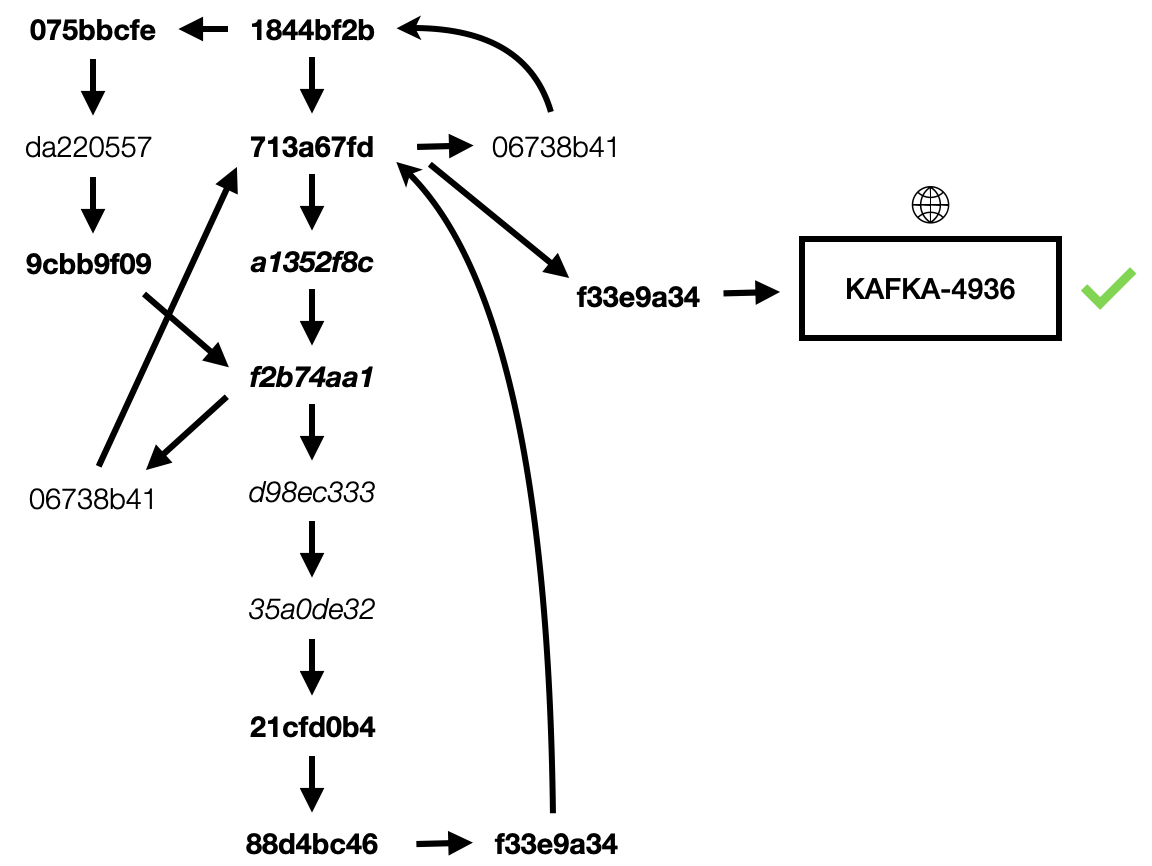
\includegraphics[width=5.5cm]{./images/graph-sample-A.png}}}%
  \qquad
  \subfloat[\centering \participant{H}'s commit history exploration in answering question B1 without Intelligent History. \label{subfig:Exploration-Graph-B}]{{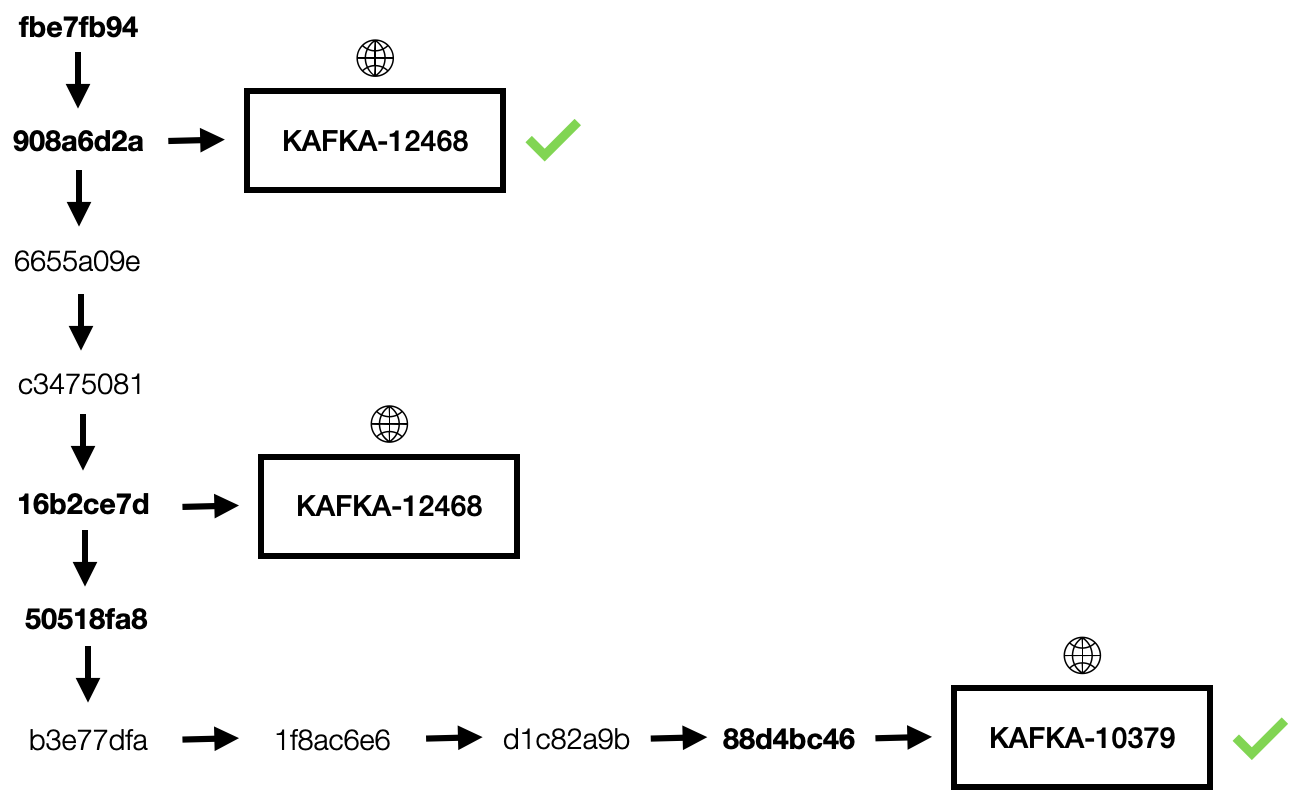
\includegraphics[width=5.5cm]{./images/graph-sample-B.png}}}%
  \caption{
    Commit history exploration graphs.
  }%
  \label{fig:Exploration-Graphs}%
\end{figure}

As a demonstration of how we devised themes for the participants' exhibited approaches for commit history exploration, 
\autoref{subfig:Exploration-Graph-A} illustrates the participant \participant{B}'s approach to finding 
two meaningful commits as per question B1 without using Intelligent History.
The commit history exploration graph for \participant{B} shows they examined 16 out of 45 commits.
Participant \participant{B} would examine a few commits at a time and 
backtrack to previously seen commits after gaining a broad sense of the changes made over time to the file.
We characterize the structure of the graph for \participant{B} as \textit{cyclic and backtracking}
to describe the history exploration strategy they predominantly exhibited.
Meanwhile, the commit history graph for \participant{H} shown in \autoref{subfig:Exploration-Graph-B}, 
who answered the same question without Intelligent History, shows they examined 10 out of 45 commits.
Participant \participant{H} exhibited an approach where they examined each commit sequentially in chronological order.
We characterize the structure of the graph for \participant{H} and their commit history exploration approach as \textit{linear} 
to describe the participant's sequential or chronological exploration of the commit history.

The flowchart showing the relationship between each participant's background related to looking at commits and issues,
the commit history exploration approach they used, and their preferred features 
provided by Intelligent History is presented in \autoref{fig:Flow-Chart-Individual}.
The features of Intelligent History are the actions we detailed in \autoref{sec:Implementation}, which are 
(\feature{1}) \textit{Highlight Important Changes}; 
(\feature{2}) \textit{Show Diff Metadata}; 
and (\feature{3}) \textit{Show Jira Metadata}.
We also present an aggregated version of the flowchart in \autoref{fig:Flow-Chart-Aggregate} 
and a tabular form in \autoref{tab:Flow-Chart-Tabular}.

\begin{figure}[h]
  \centering
  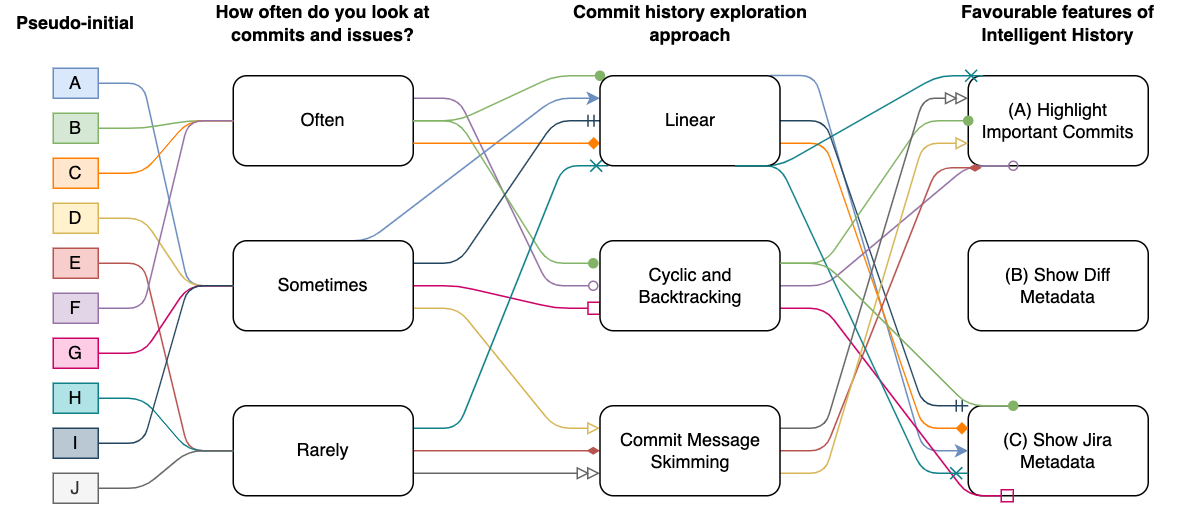
\includegraphics[width=12cm]{./images/flow-chart-ind.png}
  \caption{
    The relationship between how often a participant looks at commits and issues, 
    the approach they exhibited to exploring commit history overall, 
    and the feature of Intelligent History they were most partial to.
  }
  \label{fig:Flow-Chart-Individual}
\end{figure}

\begin{figure}[h]
  \centering
  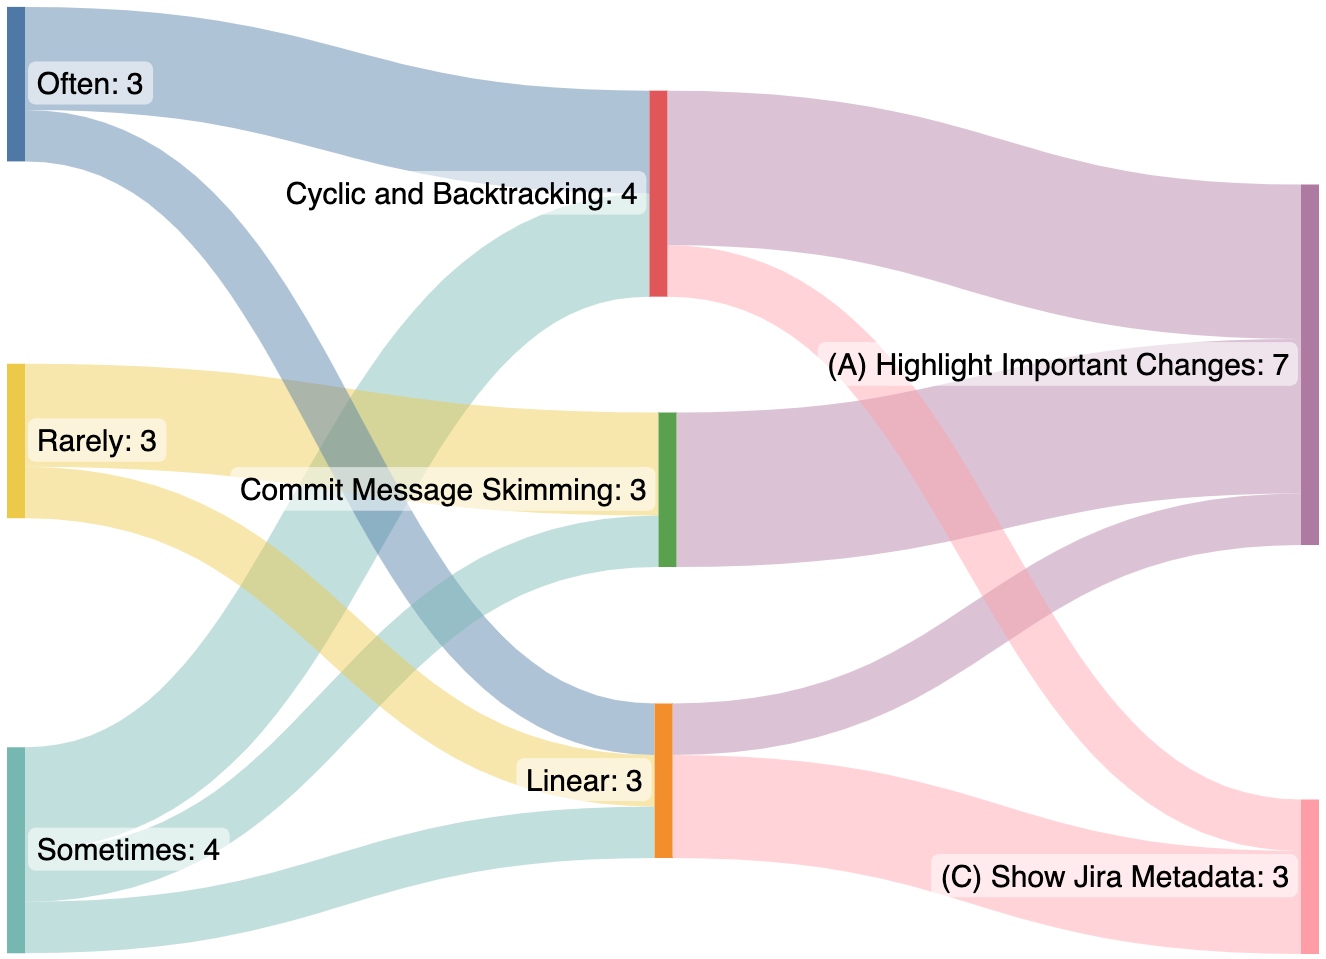
\includegraphics[width=8cm]{./images/flow-chart-aggr.png}
  \caption{
    An aggregation of the participants that fall into each of the categories from \autoref{fig:Flow-Chart-Individual} and \autoref{tab:Flow-Chart-Tabular}
  }
  \label{fig:Flow-Chart-Aggregate}
\end{figure}

Over half of the participants, 6 out of 10, preferred feature (\feature{1}) from Intelligent History the most,
whereas the other 4 participants preferred feature (\feature{3}).
Notably, all 5 of the participants who received question set A to answer with Intelligent History 
responded most positively to commit history highlighting in (\feature{1}) as a feature \participants{BDFHJ}, 
whereas 4 out of the 5 participants who received question set B to answer with Intelligent History 
responded most positively to gaining quick access to Jira issue information within the \entity{IDE} in (\feature{3}) as a feature \participants{ACGI}.
This signifies some degree of correlation between the question set and the participants' most preferred features of Intelligent History.

None of the participants chose feature (\feature{2}), though we anticipated this outcome as (\feature{2}) 
was provided to give the user context as to how Intelligent History highlights commits in (\feature{1}).
Of the 3 participants who stated that they often look at commits and issues, none demonstrated \textit{commit message skimming} 
as a strategy for exploring commit history.
Similarly, of the 3 participants who rarely look at commits and issues, none of them employed a commit history exploration approach 
that could be described as \textit{cyclic and backtracking}.
There does not appear to be any concrete associations between the background of a participant with regard to looking at commits and issues,
and their exhibited approach to exploring commit history.

On the relationship between the commit history exploration approach a participant exhibited and their preferred feature from Intelligent History,
3 out of 4 participants who demonstrated a cyclic and backtracking approach expressed preference for (\feature{1}),
while all 3 participants who exhibited a \textit{commit message skimming} strategy were most partial to (\feature{3}).

\begin{landscape}
  \begin{table}
    \footnotesize
    \caption{
      A tabular form of \autoref{fig:Flow-Chart-Individual}.
    }
    \centering
    \begin{tabular}{@{}c|ccl@{}}
      \toprule
      \textbf{Pseudo-initial} & \textbf{\begin{tabular}[c]{@{}c@{}}How often do you look\\ at commits and issues?\end{tabular}} & \textbf{\begin{tabular}[c]{@{}c@{}}Commit history\\ exploration approach\end{tabular}} & \multicolumn{1}{c}{\textbf{\begin{tabular}[c]{@{}c@{}}Favourable feature of\\ Intelligent History\end{tabular}}} \\ \midrule
      A                       & Sometimes                                                                                       & Cyclic and Backtracking                                                                & (\feature{3}) Show Jira Metadata                                                                                           \\ \midrule
      B                       & Often                                                                                           & Cyclic and Backtracking                                                                & (\feature{1}) Highlight Important Changes                                                                                  \\ \midrule
      C                       & Often                                                                                           & Linear                                                                                 & (\feature{3}) Show Jira Metadata                                                                                           \\ \midrule
      D                       & Sometimes                                                                                       & Commit Message Skimming                                                                & (\feature{1}) Highlight Important Changes                                                                                  \\ \midrule
      E                       & Rarely                                                                                          & Commit Message Skimming                                                                & (\feature{1}) Highlight Important Changes                                                                                  \\ \midrule
      F                       & Often                                                                                           & Cyclic and Backtracking                                                                & (\feature{1}) Highlight Important Changes                                                                                  \\ \midrule
      G                       & Sometimes                                                                                       & Cyclic and Backtracking                                                                & (\feature{3}) Show Jira Metadata                                                                                           \\ \midrule
      H                       & Rarely                                                                                          & Linear                                                                                 & (\feature{1}) Highlight Important Changes                                                                                  \\ \midrule
      I                       & Sometimes                                                                                       & Linear                                                                                 & (\feature{3}) Show Jira Metadata                                                                                           \\ \midrule
      J                       & Rarely                                                                                          & Commit Message Skimming                                                                & (\feature{1}) Highlight Important Changes                                                                                  \\ \bottomrule
    \end{tabular}
    \label{tab:Flow-Chart-Tabular}
  \end{table}
\end{landscape}

%%%%%%%%%%%%%%%%%%%%%%%%%%%%%%%%%%%%%%%%%%%%%%%%%%%%%%%%%%%%%%%%%%%%%%

\subsection{RQ1}
\label{subsec:RQ1}

\RQ{1}{Can we automatically identify the commits that software developers would want to examine?}

The underlying approach to commit highlighting involved the construction of regular expression patterns 
as a minimal set of rules for distinguishing commits containing non-essential changes.
We ask this research question to assess the performance of the underlying approach 
used in Intelligent History's commit highlighting feature (\feature{1}).

In addition to the number of unique commits a participant examined as part of answering a question,
we computed the proportion of those commits that would be highlighted commits according to Intelligent History.
We did this to observe:
(1) whether a large proportion of commits a participant inspects would be considered as important using Intelligent History
and (2) the influence of Intelligent History's commit highlighting on which commits a participant chooses to examine.

We found that for questions that participants completed without Intelligent History,
over half of the commits that participants examined would have been highlighted by Intelligent History.
For A1, a mean of 68.5\% of the commits that the participants examined would be highlighted commits.
For A2, a mean of 76.7\% of the commits that the participants examined would be highlighted commits.
For B1 and B2 respectively, a mean of 51.3\% and 100.0\% of the commits that the participants examined would be highlighted commits.
This indicates that in cases where Intelligent History is not used and therefore does not influence the commits participants examine,
we observe a degree of overlap between the commits that participants choose to further investigate and the commits that Intelligent History highlights.

When participants had access to Intelligent History,
nearly 100.0\% of the commits they examined for a question were highlighted commits.
For A1, a mean of 100.0\% of the commits that particpants who used Intelligent History examined were highlighted commits.
For A2, the mean was 97.1\% of the commits.
Similarly for B1 and B2, a mean of 100.0\% of the commits that participants who used Intelligent History examined were highlighted commits.
According to these results, we make the observation that highlighted commits heavily 
influenced how participants selected commits from the commit history for further investigation, as
nearly all of the commits that participants chose to inspect from the commit history were commits that Intelligent History highlighted.
While this is not sufficient evidence to comment about the agreement from participants on the commits Intelligent History
chooses to highlight and not highlight,
we observe that participants did not choose to examine the commits Intelligent History did not highlight
for 3 out of 4 questions asked in the user study.

In the interviews we conducted, 
several participants commented on how commit highlightling de-emphasized ``minor'' changes from the history \participants{BDEFH}.
Although participants were not asked to validate the commits that Intelligent History chose to highlight and to fade out from the commit history, 
participant \participant{B} expressed agreement with the highlighting, 
noting that the faded commits ``\textit{do not seem to be useful for this file [the \class{Topology} class] at all}.''

\begin{summary}[RQ1]
  An automatic approach based on using regular expressions applied to commit diffs 
  can support software developers exploring a commit history 
  by distinguishing the non-essential commits in a commit history,
  thereby helping developers focus their attention on other commits.
\end{summary}

%%%%%%%%%%%%%%%%%%%%%%%%%%%%%%%%%%%%%%%%%%%%%%%%%%%%%%%%%%%%%%%%%%%%%%

\subsection{RQ2}
\label{subsec:RQ2}

\RQ{2}{Does highlighting important commits help software developers explore a file’s revision history more efficiently?}

We define the measure for efficiency as the proportion of commits from a file's commit history that a developer must examine before obtaining the answer to questions about the intent behind code changes.
We found highlighting to distinguish non-essential commits from other commits in a history
did lead to a reduced percentage of commits examined when exploring a file's commit history 
for questions related to identifying meaningful source changes 
and the rationale behind those changes when the developer must navigate a broad commit history for a file. 
This is evidenced by the participants who used Intelligent History to answer questions A2 and B1 
as they examined a significantly smaller proportion of a given file's commit history 
to obtain the code ratianale information needed for answering the questions asked in the user study.

\subsubsection{Navigating a Broad Commit History}

We first discuss the results for questions from the questions sets in \autoref{tab:Question-Sets},
where there was a significant difference between
the mean proportion of commits examined between the group of participants who used Intelligent History with a question 
and the group who did not use Intelligent History.

For question A2, participants who used Intelligent History examined a mean of 19.9\% of the commit history for the \class{Topology} class,
while participants who did not use Intelligent History examined a mean of 39.1\% of the same commit history. 
% Moreover, of the participants who used Intelligent History and the proportion of commits they examined,
% a mean of 97.1\% of the commits they examined were highlighted commits.
% For the group that did not use Intelligent History, a mean of 76.1\% of the commits they examined 
% would have been highlighted commits under feature (\feature{1}) \textit{Highlight Important Changes} from Intelligent History.
To answer A2, participants needed to find a commit that introduced further \code{addSink} method overloads later in the commit history as participants were informed that the initial commit in the commit history for the \class{Topology} class introduced a set of overloaded \code{addSink} methods to begin with.
The specific commit which does this is commit \commitref{f33e9a34}{https://github.com/apache/kafka/commit/f33e9a346e22e29bb66e0ea0f3442903d136ca67} with the following commit message title:

\begin{center}
  \jira{KAFKA-4936:}{Add dynamic routing in Streams (\#5018)} 
\end{center}

Participants were not expected to be able to identify this commit based on its commit message title alone.
However, participants intuited to locate a particular commit that introduced further overloads later in the history 
to understand why additional overloads were introduced to the \class{Topology} class.
This could be done through examining diffs of potentially interesting commits for commits 
that were made after the initial commit in the \class{StreamsBuilder} commit history.

Interestingly, all of the participants who used Intelligent History to answer question set A 
responded most positively to feature (\feature{1}) from Intelligent History \participants{BDFHJ} 
(see \autoref{tab:Participants} and \autoref{tab:Flow-Chart-Tabular}).
This could have been because the group of participants who answered question set B first without Intelligent History 
and question set A after with Intelligent History would be able to reflect on how Intelligent History could have been useful for the other question set.
Participants commented on the utility of commit history highlighting for focusing their attention on commits that were highlighted 
and ignoring non-highlighted commits, which they regarded as ``irrelevant'' or ``minor'' \participants{BF}.
Participant \participant{B} said:

\begin{quote}
  When I think to what I have to do at work, 
  often you don’t know what kind of modification you’re looking for. 
  Especially when automated tests break or something, 
  you’re going to be looking for something that is very recent and if you’re on a popular file, 
  there might be a lot of commits. 
  But with this [commit history highlighting], 
  you’d be able to easily filter out things that actually made differences rather than negligible changes.
\end{quote}

Specifically regarding answering A2, participant \participant{H} stated:

\begin{quote}
  [Highlighting commits] was amazing for speeding up what I had to search for. 
  Especially, in finding that sink issue [in A2], if I didn’t have the pencil [Highlight Important Changes feature], 
  I think I would have gone through all the commits backwards and just try to see what the diffs are 
  but it removed a bunch of the ones that it [Intelligent History] deemed not useful and it ended up being correct so I just skipped over a bunch [of commits].
\end{quote}

Comparing their experiences for answering the question set without and with Intelligent History, 
participants commented on the effect of commit history highlighting making commit history exploration faster by reducing the amount of irrelevant commits they would have examined \participants{DFHJ}.
Participant \participant{D} mentioned: 
``\textit{[The highlighting] allowed for me to skim through the necessary commits a lot quicker \dots and visually reduces the amount of clutter I had to look at.}''
In a similar vein, participant \participant{J} commented:
``\textit{[The highlighting] removed the obvious minor changes that I didn’t really need to look at.}''

Meanwhile, in answering question B1, participants who used Intelligent History examined a mean of 15.6\% of the commit history for the \class{StreamsBuilder} class,
whereas participants who did not use Intelligent History examined a mean of 33.3\% of the same commit history.
% Of the commits that the group who used Intelligent History examined for answering B1, a mean of 100.0\% of the commits were highlighted commits.
% For the group who did not use Intelligent history to answer B1, a mean of 51.3\% of the commits they examined would have been highlighted commits if they used Intelligent History.
Question B1 necessitated for the participants to examine commits and diffs in the \class{StreamsBuilder} commit history to try to identify meaningful source code changes that were made to the class.
We clarified a meaningful source code change to be a commit that improves some functionality or behaviour in the class and expected participants to utilize the diffs and intent of a change's author to justify their answer.
Despite the group of participants who used Intelligent History to answer B2 looking at less than half the proportion of commits that the group who did not use Intelligent History looked at (15.6\% compared to 33.3\%),
only 1 participant emphasized commit history highlighting as a feature that made the strongest impression on them \participants{E}, 
whereas the remaining 4 participants showed a preference for feature (\feature{3}) of Intelligent History instead \participants{ACGI}.
Participant \participant{E} said:

\begin{quote}
  I think that the biggest benefit [of Intelligent History] was especially removing minor changes. 
  It’s [the \textit{Highlight Important Changes} feature] really handy; it filters a bunch of -- not garbage -- but noise in the commit history. 
  With just this single feature [commit history highlighting], it’s already worth using the plugin.
\end{quote}

On the commit history highlighting feature, participant \participant{A} stated:

\begin{quote}
  I liked the highlighting. 
  It’s nice to not look at so many commits. 
  [\dots] Looking at the history without the highlighting is kind of overwhelming because it’s just like ``oh my god, this is a flood of commits, 
  what are we going to do?'' 
  but when you get rid of the less important ones, it’s [\dots] much more manageable.
\end{quote}

Of the 6 participants that expressed preference for feature (\feature{1}), 
2 employed a commit history exploration approach that could be described as \textit{cyclic and backtracking} based on their commit history exploration graphs \participants{BF},
3 used commit message skimming \participants{DJ}, and 1 used a linear approach \participants{H}.
Thus, we find less of a relationship between a participant's software history exploration approach and their preference for feature (\feature{1}).

\subsubsection{Locating Rationale for a Code Fragment}

As captured from the results of the $t$-test in \autoref{tab:t-test}, 
there was no evidence to support the claim of a significant difference in the proportion of commits examined by the groups for answering questions A1 and B2.
Both questions A1 and B2 are similar in nature as they require the participant to inspect a specific section of code given by line numbers and attempt to locate commits relevant to these code segments.
Participants who vocalized familiarity with using \entity{git} ``blame'' were shown and permitted to use the native ``Show History for Selection'' feature in IntelliJ to narrow down the commits to look at.
This native feature enabled participants to view a subset of commits affecting selected fragments of source code.

In recognition of the suitability of commit history highlighting for certain types of questions,
2 participants who received question set B first without Intelligent History and question set A 
after with Intelligent History commented on their desire to use Intelligent History's commit highlighting feature for question B1
if they were to re-do the question because B1 required exploration of a larger commit history \participants{BD}.
Participant \participant{B} mentioned:

\begin{quote}
  [For] the questions [I was] asked [\dots] the plugin didn’t help that much. 
  For example, one of the questions in the \class{StreamsBuilder} class was to look for commits that improve things, 
  so I feel like if I had to re-do that task, then using the highlighting would have been useful.
\end{quote}

For question A1, 6 participants used the ``Show History for Selection'' feature \participants{CEFHIJ},
and the other 4 participants manually found the commit that introduced the change and contained the rationale information by reading the commit mesage subjects and using the chronological information based on other commit timestamps \participants{ABDG}.
For question B2, the failure to reject the null hypothesis may be attributed to the fact that the commit \commitref{e09d6d79}{https://github.com/apache/kafka/commit/e09d6d796f5a0b840519021d7f6435c65f88a60a} which contains the information necessary for answering this question has the message title: 

\begin{center}
  \jira{KAFKA-7027:}{Add overloaded build method to StreamsBuilder (\#5437)} 
\end{center}

Hence, participants familiar with using version control tools for similar questions encountered in every day work would be able to quickly narrow down the commit needed to answer the question without requiring traversal of the file's commit history.
Due to the nature of A1 and B2 and the limited impact of commit highlighting on the participants' experience with answering these questions,
our samples are insufficient for obtaining evidence to show a significant difference in commit history exploration efficiency between the group that does not use Intelligent History and the group that does use Intelligent History for questions that ask about specific sections of code from a Java class.

Thus, based on our analysis of A2 and B1 where there was a significant difference in 
the proportion of commits examined by participants using Intelligent History, 
we observe that participants who use Intelligent History with its commit highlighting feature 
look at a smaller proportion of commits from a file's commit history when answering questions related to
identifying and finding meaningful source code changes over a broad commit history.
In support of this observation, 
participant \participant{A} expressed a beneficial use case of commit history highlighting 
for reducing the number commits a software developer examines:

\begin{quote}
  If I was trying to get a sense of major changes in a file, like say there was an issue that came up in a file and I’m looking for where it could have gotten introduced, 
  then that [highlighting commits] would be very useful because it gets rid of all the changes that don’t matter. 
\end{quote}

\begin{summary}[RQ2]
  Commit history highlighting can support software developers in efficiently 
  exploring commit history for code rationale information 
  by examining a smaller proportion of the commits in a file's commit history.
  Commit history highlighting makes identifying and searching for meaningful source code changes 
  across a broad commit history more efficient but has less impact when trying to find rationale information for specific code segments in a file.
\end{summary}

%%%%%%%%%%%%%%%%%%%%%%%%%%%%%%%%%%%%%%%%%%%%%%%%%%%%%%%%%%%%%%%%%%%%%%

\subsection{RQ3}
\label{subsec:RQ3}

\RQ{3}{How useful is direct integration of issue information in the IDE for helping a developer search for code rationale information?}

In our implementation of feature (\feature{3}), we integrated a view of a Jira issue's title, description, reporter, assignee, priority,
and metadata information related to the number of comments and linked issues to give the plugin user a signal 
of how interesting a Jira issue might be for further examination.
We found the utility of direct integration of issue information 
to be dependent on a participant's background with examing commits and issues,
and the software history exploration approach they employ.
The usefulness of direct integration of issue information is also dependent on 
\emph{what} information is extracted from an issue and how it is presented in the \entity{IDE}.

\subsubsection{Breadth and Contextualization}

We anticipated question B1 to require the most application switching between the \entity{IDE} 
and browser and to have the highest number of mean Jira issues viewed.
This is because B1 requires participants to examine the diffs of commits to ensure they consist of source code changes 
that comply with the criteria of improving some functionality or behaviour in the \class{StreamsBuilder} class.
Participants were also asked to justify their answer by finding supporting evidence for the commit author's intent behind their change.

The participant group who did not use Intelligent History with B1 had a mean number of application switches of 2.0,
while the group who did use Intelligent History had a mean number of application switches of 0.8.
The group who did not use Intelligent History with B1 viewed a mean of 2.0 Jira issues,
while the group who did use Intelligent History with B1 viewed a mean of 3.2 Jira issues.
We observe that participants who used Intelligent History for locating meaningful source code changes and finding the code rationale behind the changes
were able to view more Jira issues with slightly less application switches than participants who did not use Intelligent History for the same task.

Coincidentally, 4 of the 5 participants from the group that answered question set B with 
Intelligent History actually favoured feature (\feature{3}) \textit{Show Jira Metadata} \participants{ACGI}.
Participant \participant{A} commented:

\begin{quote}
  I thought that the Jira integration was very helpful because you don’t have to go to Jira to look at all the stuff and deal with Jira. 
  It’s [the issues] just in the \entity{IDE} which is nice; it’s [the plugin] quick and fast.
\end{quote}

Participant \participant{J} mentioned:

\begin{quote}
  Without the plugin, it was a little more annoying and time-consuming opening up the browser, 
  looking for all of the issues, 
  whereas with the plugin, 
  it was already there [in the \entity{IDE}] and I can just take a quick look and see if it [the commit] 
  might be relevant and I can take a deeper look if needed.
\end{quote}

Of the 4 participants who favoured (\feature{3}), none demonstrated a commit message skimming approach to exploring commit history in the user study.
Only 1 of the participants reported looking at commits and issues often \participants{C},
while 3 participants reported sometimes \participants{AGI}.
Perhaps unsurprisingly, none of the participants who favoured (\feature{3}) reported looking at commits and issues rarely.

While we observed there to be some notable difference in the group that used Intelligent History for question B1 and the group that did not use Intelligent History for the same question,
there is less notable difference with question B2.
Hence, we find that the primary question responsible for this bias is question B1.
Given the nature of B1, we find direct integration of Jira issue information within the \entity{IDE} 
to be useful for broad search and exploration of a commit history.
As participant \participant{E} stated:
``\textit{[The Jira issue integration] helps you contextualize the code change in a commit really quick.}''
However, direct issue integration is potentially less useful for those with an approach based on skimming commit messages.

\subsubsection{Issue Content and Presentation}

We found 2 participants mentioned a preference to see the full Jira issue information contextualized in the browser interface \participants{DF}.
While participant \participant{F} mentioned that they were accustomed to viewing Jira issues in the browser \participants{F},
participant \participant{D} stated that they had a preference to view all items associated with a Jira issue, including all linked issues and pull requests:
``\textit{When I’m looking at a Jira ticket, I look at everything associated with the ticket to try to get a much broader context.}''
On the other hand,
participant \participant{E} stated that they did not look at parts of an issue beyond the description and a few comments:
``\textit{I wouldn’t bother that much with looking at the issue for other things like discussion, other than the description and perhaps the last two comments, 
I wouldn’t look much further than that}.''
We found there may be some limitations related to \emph{what} information was presented in the integrated view of the Jira issue in the \entity{IDE}
and the personal preferences and habits of the user.

Similar in sentiment, participant \participant{G}, who favoured (\feature{3}), noted the hyperlinking of Jira issues for each commit
was most helpful to them in the user study.
\participant{G} observed that since some of the Jira issues included code fragments, it was difficult to read them in the \entity{IDE}.
This indicates the presentation of the issue information may be an impediment to its utility.

\begin{summary}[RQ3]
  Direct integration of issue information can help software developers contextualize source code changes 
  and access the information in more issues than without,
  particularly when searching for interesting or meaningful changes across a file's commit history.
  However, the utility of direct integration of issue information is dependent on users' preferences preferences and habits 
  with regard to the content they prefer to see from issues and how they would like them to be presented.
\end{summary}

%%%%%%%%%%%%%%%%%%%%%%%%%%%%%%%%%%%%%%%%%%%%%%%%%%%%%%%%%%%%%%%%%%%%%%

\section{Threats to Validity}

\subsection{Construct Validity}

The size of the question sets we asked is a threat to construct validity.
Due to the laboratory setting of the user study and the time estimated for participants to perform environment setup,
be introduced to the Apache Kafka project, Jira, the IntelliJ IDEA IDE, and the Intelligent History plugin,
we restricted the number of questions asked to account for a reasonable total estimated session time.
We formulated small sets of questions to relieve participants from a time limit 
and give them the freedom to explore the commit histories, inspect individual commits, and read Jira issues at their own pace.
Although the small quantity of questions allowed us to observe the participants closely for each information-finding question,
we risk the ability to observe the consistency of the participants' commit history exploration strategies
 across larger sets of questions to use without and with Intelligent History.

\subsection{Internal Validity}

The presence of an observer in the user study sessions means the participants' behaviour, opinions, 
and feedback about the Intelligent History plugin are subject to the Hawthorne effect,
which threatens internal validity.
The presence of an observer could have caused participants to deviate from their regular work habits 
as the participants might have formed an expectation about how to behave or explore the commit history.
We attempted to mitigate this effect by minimizing observer interjections during the sessions, 
though prior to the study, participants were encouraged to think aloud to describe their strategies 
to finding the information necessary to answer the questions.
We also provided participants with the opportunity to self-report, clarify their actions, 
and provide feedback on their experience with participating in the user study during their follow-up interviews.

The introduction of the Intelligent History plugin to the participant could be a threat to internal validity.
After being introduced to the features of Intelligent History, 
the participant could be biased to use or conduct themselves in the study a certain way.
For example, toggling feature (\feature{1}) \textit{Highlight Important Changes} 
results in highlighting the commits in a commit history to distinguish less important commits from potentially more important commits.
If we initially introduced Intelligent History to a participant for their first question set,
and asked the participants to work on a second question set without Intelligent History,
they may have tried to answer the questions in the same way they would have if they had access to Intelligent History.
Consequently, in the follow-up interview, participants may have felt biased to feel a certain way about the plugin.

We tried to mitigate bias in how a participant expects to use Intelligent History and the utility of Intelligent History to a particular question set 
by alternating the order of the questions each participant received and fixing the use of the plugin to the second question set that each participant receives.
By providing each participant with a different set of questions to answer with and without Intelligent History respectively,
we also mitigate the threat to internal validity of a participant having exposure to the same questions prior to using Intelligent History.
Though the participants might have felt biased after using the plugin,
we would still be able to retain and collect data about how the participant approached exploring the commit history and answering the questions without being made aware of the plugin's features initially.

The experience of the participants with regard to having worked on a project that uses an issue tracking system and closely associating issues to commits impacts internal validity.
We tried to mitigate the impact of participant experience on internal validity by formulating questions that would require participants to justify their answers using source code and Jira issue information to
encourage participants to view Jira issues.

\subsection{External Validity}

The sample size of 10 participants affects the generalizability of our results and is a threat to external validity.
Collecting data for a larger sample size may lead to more robust conclusions about the relationship 
between a developer's experience with looking at issues and commits,
the commit history exploration strategy or strategies they employ, 
and the aspects of Intelligent History they found to be most useful.
Nevertheless, a strength of our participant pool is representation as we obtained samples from 4 students and 6 full-time developers from different companies,
representing a combination of participants from academia and industry.

A field study to investigate and evaluate the performance of the approaches in Intelligent History might also be needed to improve generalizability.
Rather than designing sets of questions pertaining to the commit history and issues available in one open-source repository,
which was Apache Kafka in our user study,
a field study to investigate how developers explore commit history with and without Intelligent History in the wild 
could lead to a more robust model for determining non-essential and essential commits,
as well as gain a deeper understanding of how often developers use issues from an issue tracking system and how they prioritize the information in an issue.

%%%%%%%%%%%%%%%%%%%%%%%%%%%%%%%%%%%%%%%%%%%%%%%%%%%%%%%%%%%%%%%%%%%%%%
\endinput

Any text after an \endinput is ignored.
You could put scraps here or things in progress.